\begin{figure}[t]
\centering
\begin{subfigure}[t]{0.24\linewidth}
    \centering
    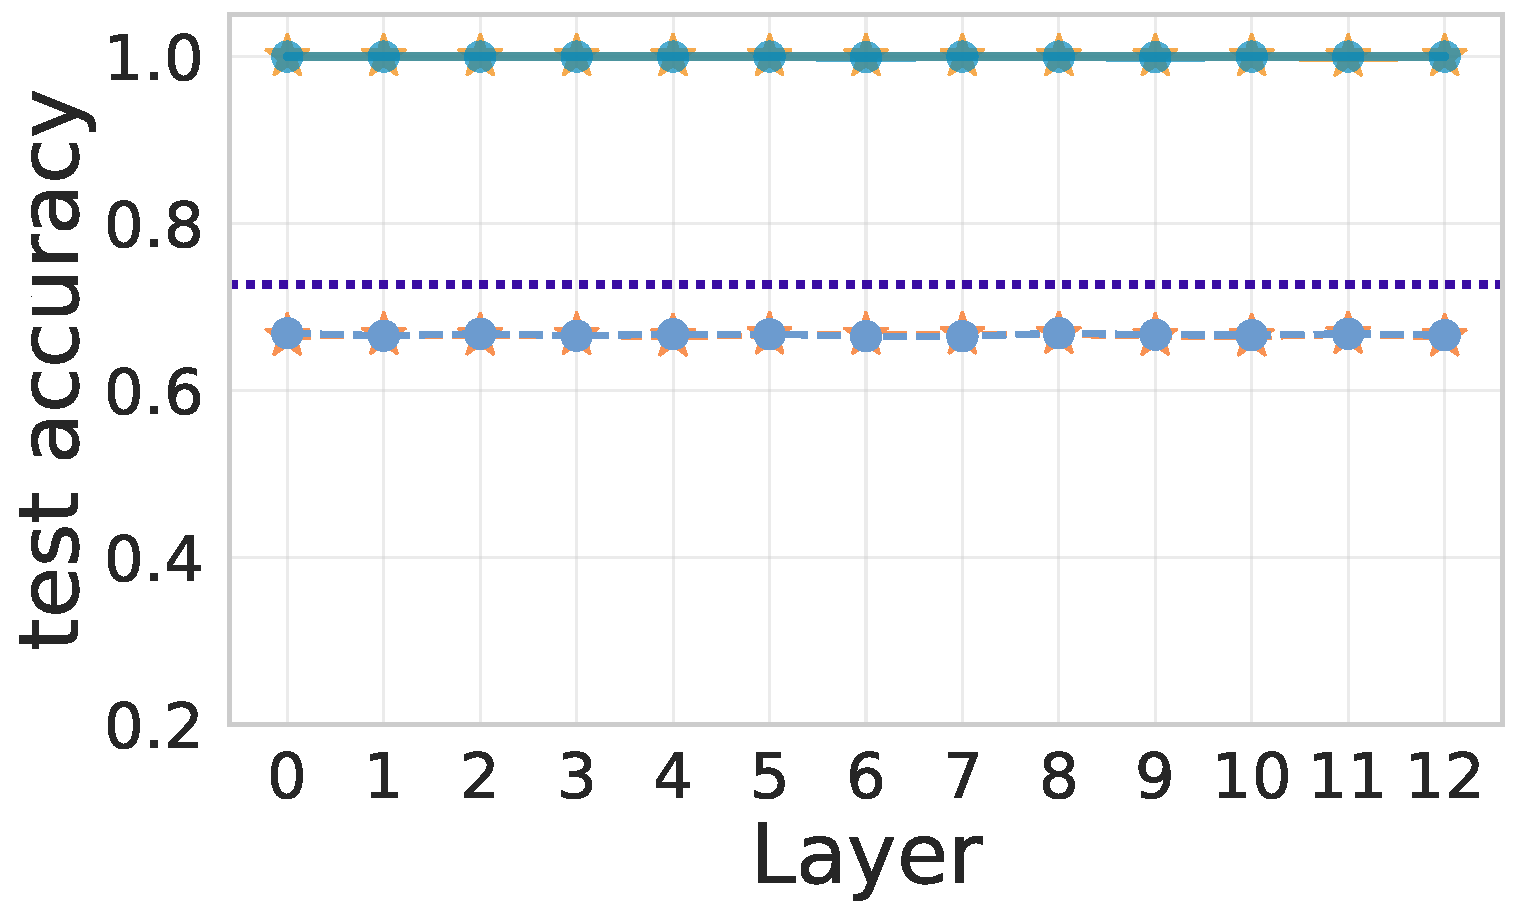
\includegraphics[width=\linewidth]{results_combined/atom_type.pdf}
    \subcaption{atom type}
    \label{fig:acc-all-atom-type}
\end{subfigure}\hfill
\begin{subfigure}[t]{0.24\linewidth}
    \centering
    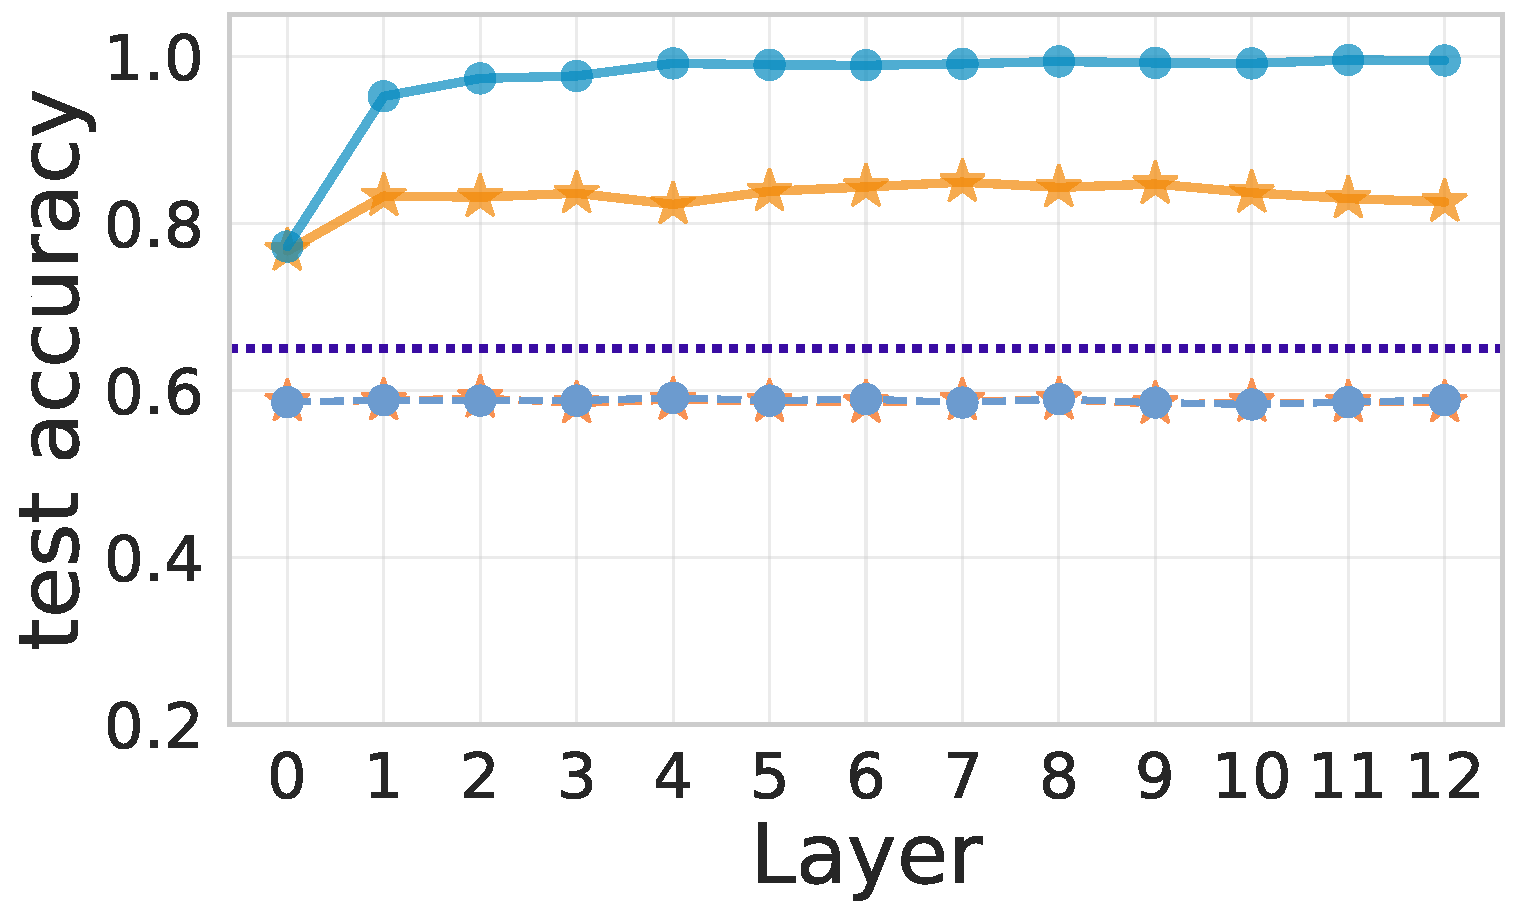
\includegraphics[width=\linewidth]{results_combined/hybridization.pdf}
    \subcaption{hybridization}
    \label{fig:acc-all-hybridization}
\end{subfigure}\hfill
\begin{subfigure}[t]{0.24\linewidth}
    \centering
    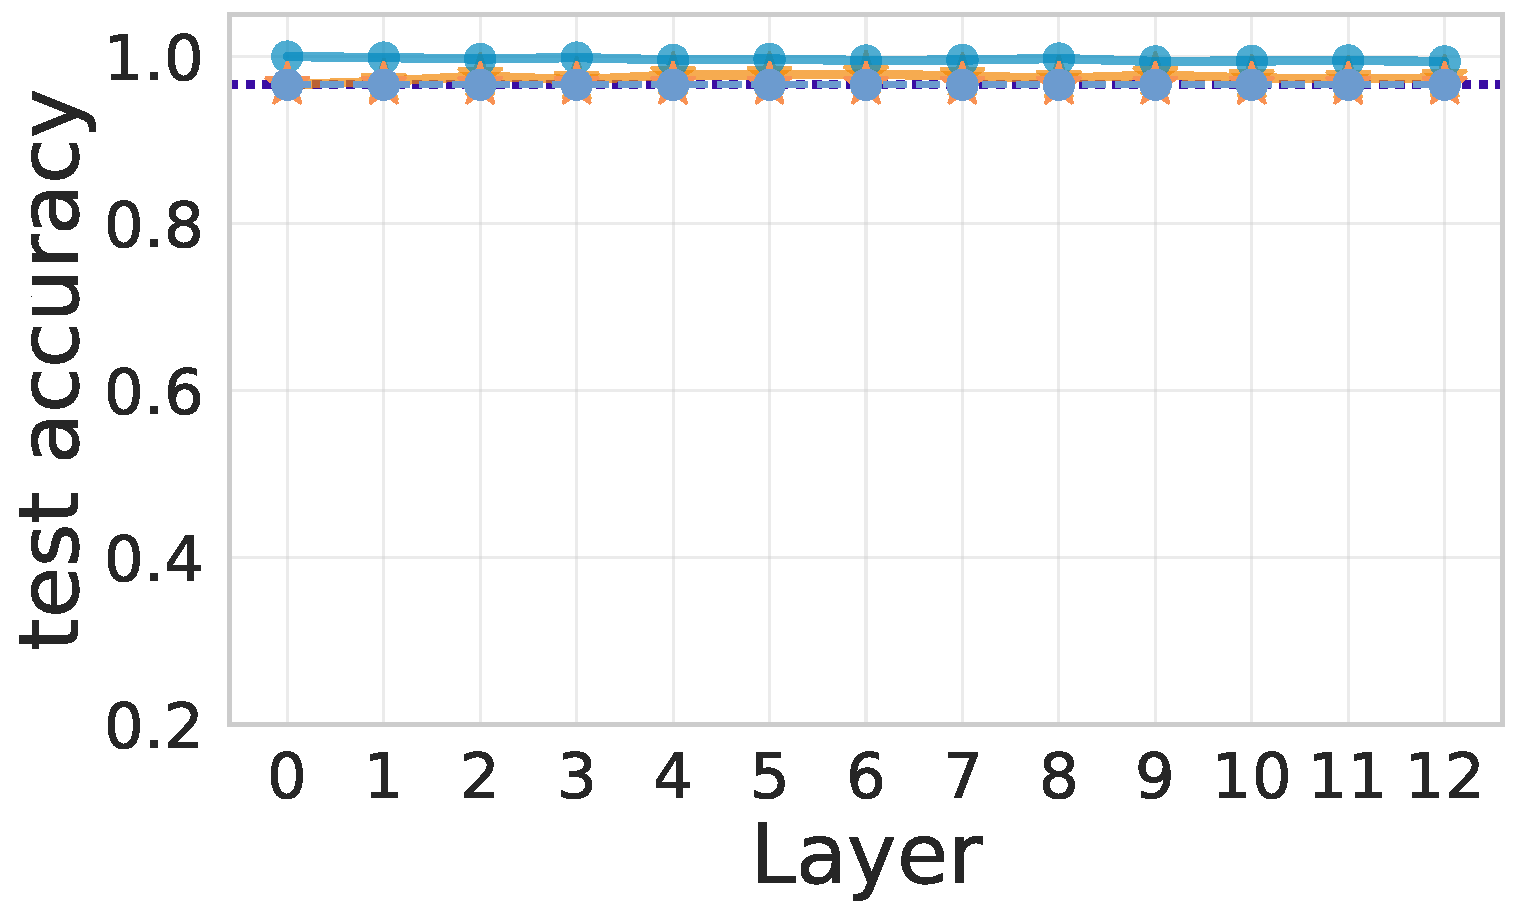
\includegraphics[width=\linewidth]{results_combined/formal_charge.pdf}
    \subcaption{formal charge}
    \label{fig:acc-all-formal-charge}
\end{subfigure}\hfill
\begin{subfigure}[t]{0.24\linewidth}
    \centering
    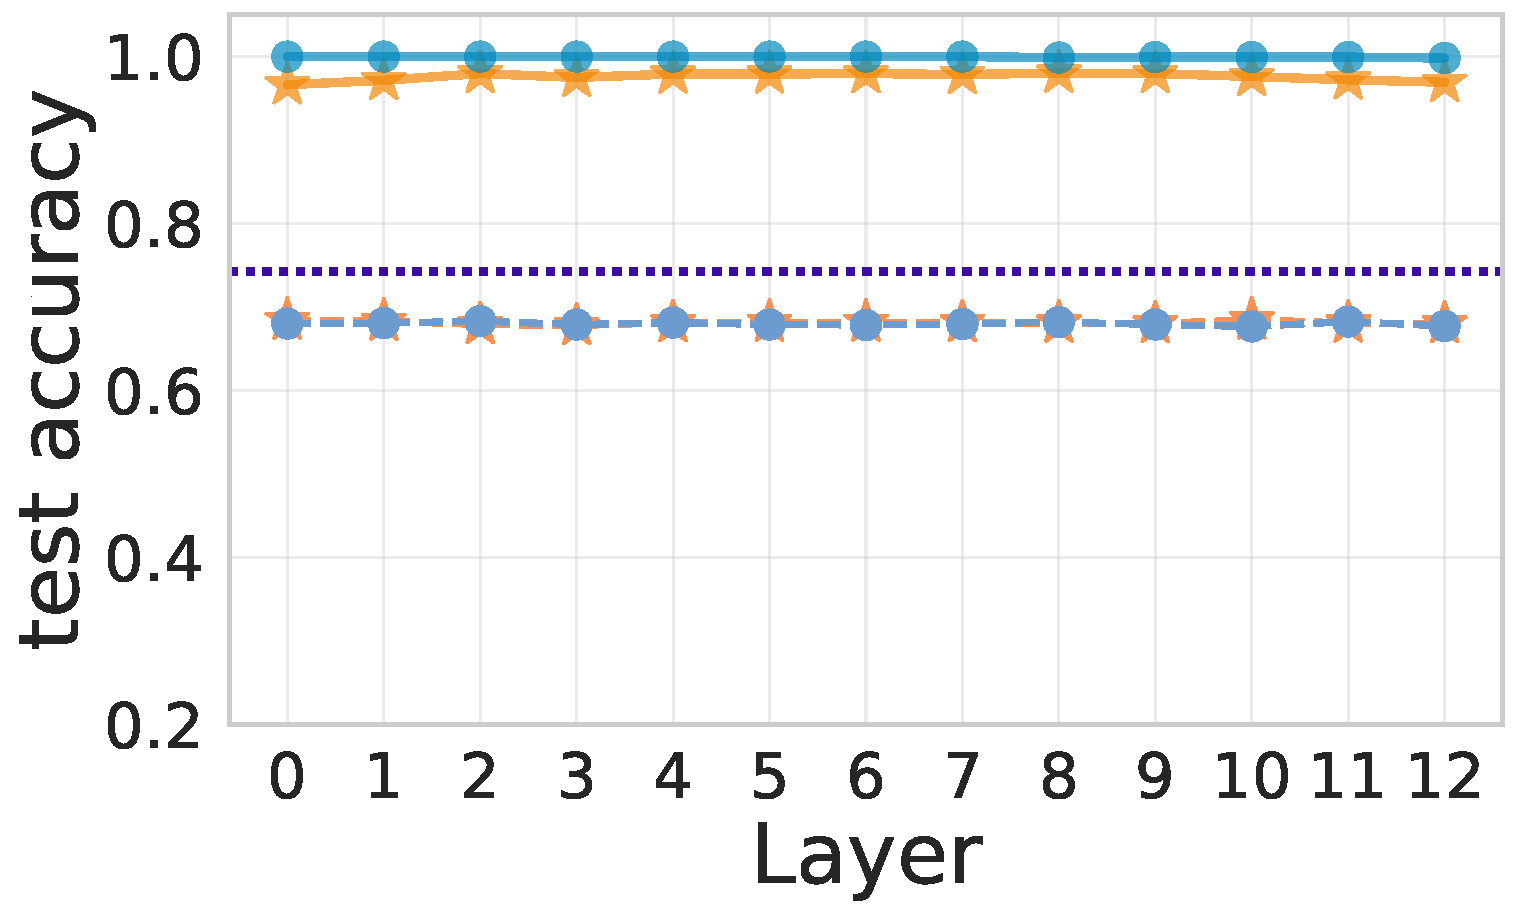
\includegraphics[width=\linewidth]{results_combined/total_valence.pdf}
    \subcaption{total valence}
    \label{fig:acc-all-total-valence}
\end{subfigure}

\vspace{0.4em}

\centerline{
\includegraphics[width=0.85\linewidth]{results_combined/legend.pdf}}

\caption{Linear-probe test accuracy per layer for the four properties not shown in the main text. Atom type (\ref{fig:acc-all-atom-type}) is surface-form and saturates at $1.0$ from layer~$0$ in both models. Formal charge (\ref{fig:acc-all-formal-charge}) is similarly close to its $0.97$ majority baseline in both models from the embedding onward. Hybridization (\ref{fig:acc-all-hybridization}) and total valence (\ref{fig:acc-all-total-valence}) are contextual and follow the same pretraining-difference shape as ring membership, degree, and chiral tag in the main text: \smi reaches near-perfect accuracy by mid-layers while \molm plateaus several points below.}
\label{fig:acc-all}
\end{figure}